\section{Results\label{sec:results}}
TODO: include blurb in the beginning that talks about how the current discrete method lacks precision with large step size and is computationally difficult with small ones.
\subsection{Setup}
\begin{enumerate}
	\item Describe baseline scenario
	\item Describe experiment setup
\end{enumerate}

\subsection{Cost Comparison with Prior Work} 
\begin{figure}
	\centering
	\makeComparisonBarChartThree{media/7_objective/costComparison5Bus5ChargersAugmented.csv}{Cost (Dollars)}{Baseline}{He et al.}{Optimized}
	\caption{Cost comparison with prior work}
	\label{fig:costComparison}
\end{figure}

\begin{enumerate}
	\item show bar plot that compares the financial results of He, baseline, and the current algorithm.
	\item show plot that shows the power vs time for the alg. and baseline
	\item show plot that shows the breakdown of uncontrolled load w/ the baseline and alg.
\end{enumerate} 

\begin{figure*}
	\centering
	\makeComparisonTotalPower{media/7_objective/optimized5Bus5ChargerAugmentedTotalPowerPlot.csv}{media/7_objective/baseline5Bus5ChargerAugmentedTotalPowerPlot.csv}{15-Minute Average Power (kW)}{Optimized}{Baseline}
	\caption{15-Minute average power for one day}
	\label{fig:totalPower}
\end{figure*}
\begin{figure*}
	\centering
	\makeComparisonPower{media/7_objective/optimized5Bus5ChargerAugmentedPowerPlot.csv}{media/7_objective/HeEtAl5Bus5ChargerAugmentedPowerPlot.csv}{15-Minute Average Power (kW)}{He et al.}{Optimized}
	\caption{Comparison between uncontrolled and bus loads}
	\label{fig:powerPlot}
\end{figure*}

\subsection{Computation Time} 

\begin{figure}
	\centering
	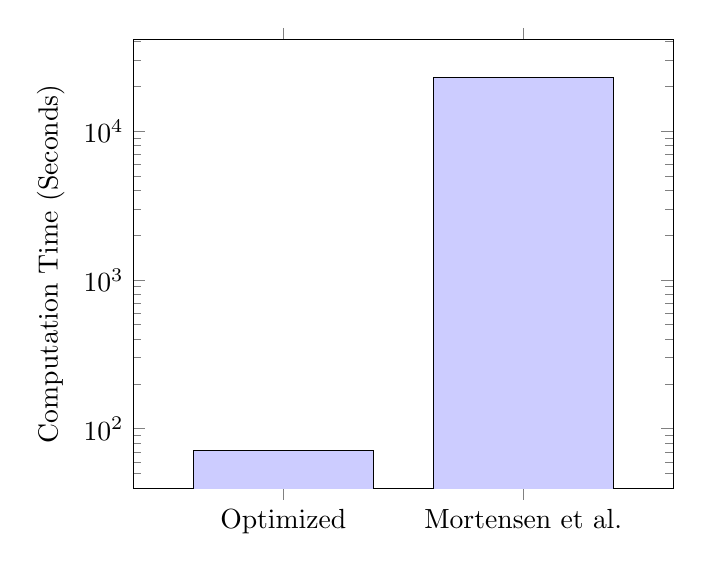
\begin{tikzpicture}
		\begin{axis}[ybar, ylabel=Computation Time (Seconds), ymode=log, xmin=0, xmax=1.8, xtick={0.5,1.3},xticklabels={Optimized, Mortensen et al.}]
			\addplot[fill=blue!20, bar width=0.6] coordinates{
			(0.5,71.187)
			(1.3,23013) 
		};
		\end{axis}
\end{tikzpicture}
%	\makeComparisonBarChartLog{media/7_objective/timeComparison5Bus5Chargers.csv}{Time (Seconds)}{Time}
\end{figure}







